\chapterOrPart{Formatting guidelines}\label{ch:formatting}
Your report or thesis will most probably contain elements such as figures, tables, numbers, units, symbols, mathematical expressions, citations and a bibliography. This chapter contains some guidelines and good practices for the proper formatting of these elements.

\section{Figures}\label{sec:formatfigures}
Figures are visual representations such as drawings, schemes, photos, charts and graphs. Every figure must be referenced in your text, preferably before the figure appears. Some important aspects of a figure are shown in \cref{fig:demofigure} and are discussed below.

\begin{frame}{A figure also requires a clear and well-written caption}
    \begin{figure}\centering
    	    \begin{tikzpicture}[scale=0.8]\node at (0,0) [above right] {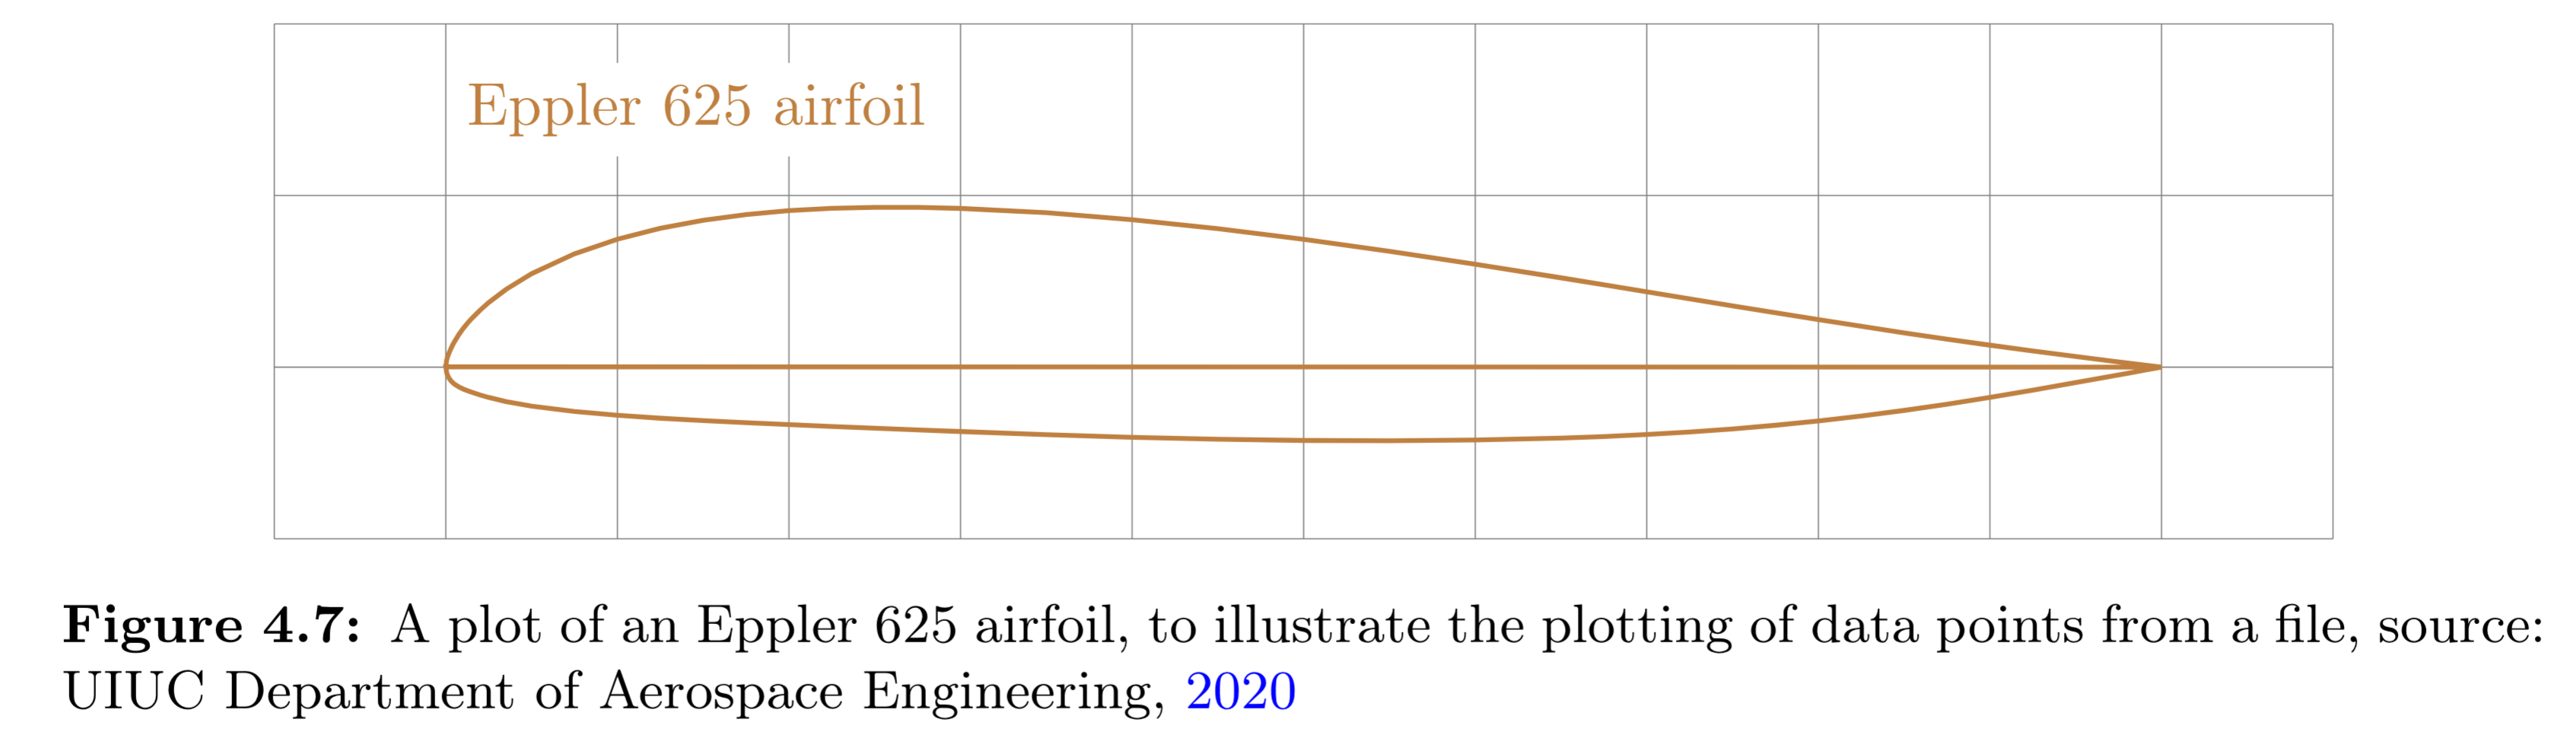
\includegraphics[width=0.9\linewidth]{figs/demofigure}};
    			%\draw [help lines] (0,0) grid (14,7); % uncomment to show grid
    			\draw [pin] (8.0,4.0)   |- + (0.5,1) node [right,align=left] {a good-quality figure};
    			\draw [pin] (0.9,1.0)   |- + (0.5,4.7) node [right,align=left] {a numbered identifier under the figure,\\referenced in the text};
    			\draw [pin] ( 2.7,0.6)  -| + (0,   -1) node [below,align=left] {a caption describing: the \textit{what}};
    			\draw [pin] (9.5 ,0.6)  -- + (0,   -1) node [below,align=left] {the \textit{so-what}};
    			\draw [pin] (15.3 ,0.6) -- + (0,   -1) node [below,align=left] {the source};
			\end{tikzpicture}
    	\caption{Some important formatting aspects of a figure and its caption}\label{fig:demofigure}
    \end{figure}
\end{frame}

First of all, your figure must be of good quality, which means that careful consideration must be given to graphical excellence and integrity (e.g. resolution, data-ink ratio, lie-factor, legend,\dots). See the excellent work of \textcite{tufte2001} and \textcite{doumont2009} for more information on these topics.

Secondly, your figure must have an unique identifier and a descriptive caption. The identifier is typically the word \textit{Figure} followed by a number. For a short report, these numbers are typically the counting numbers 1, 2, 3, etc. For a thesis or book with different chapters, the numbering of figures restarts at 1 at the beginning of each new chapter, but the chapter number is included in the figure number. See for example the number 4.7 in \cref{fig:demofigure}, which means that this is the seventh figure in chapter 4. The automatic assigning of figure numbers in \LaTeX\ is taken care of by the \cs{caption} command. If you want the caption to appear under the figure, you must place the \cs{caption} command on the last line in the figure environment. You can inspect the source code of \cref{fig:demofigure} to verify this.

A descriptive caption is a stand-alone text that must provide enough information to understand the figure, without consulting the text. The first word of the caption should be capitalized. The caption should contain a \textit{what} part and, if possible, a \textit{so-what} part. The \textit{what} part clearly explains what is shown on the figure. Try to precise and complete, it's better to have a longer caption than a short incomplete or unclear caption. The \textit{so-what} part is a statement and explains what the reader should pay attention to and/or contains a justification for showing the picture. For figures that are shown on a slide (with the beamer class), the \textit{so-what} message should be put as title of the slide, as explained in \cref{sec:slides}.

If you did not make the figure yourself, you must add the reference to the source of the figure at the end of your caption, preceded for instance by the word \verb|source:|. If the figure came from an external source but was adapted by you, you can precede the reference to the source by \verb|adapted from:|.

\subsection{Include graphical files in vector format}
To enhance the quality and scalability of graphics in documents, you should include graphical files in vector format like PDF whenever possible, rather than in bitmap format like PNG. Vector graphics maintain their sharpness and clarity at any size or resolution, making them ideal for high-quality printing and zooming in on details. In Python for instance, plots can be saved in PDF format with the command \texttt{plt.savefig(`\meta{filename}.pdf')}.

Zoom in on \cref{fig:vectorformat} and observe the difference in quality of the two plots.

\begin{figure}\centering
    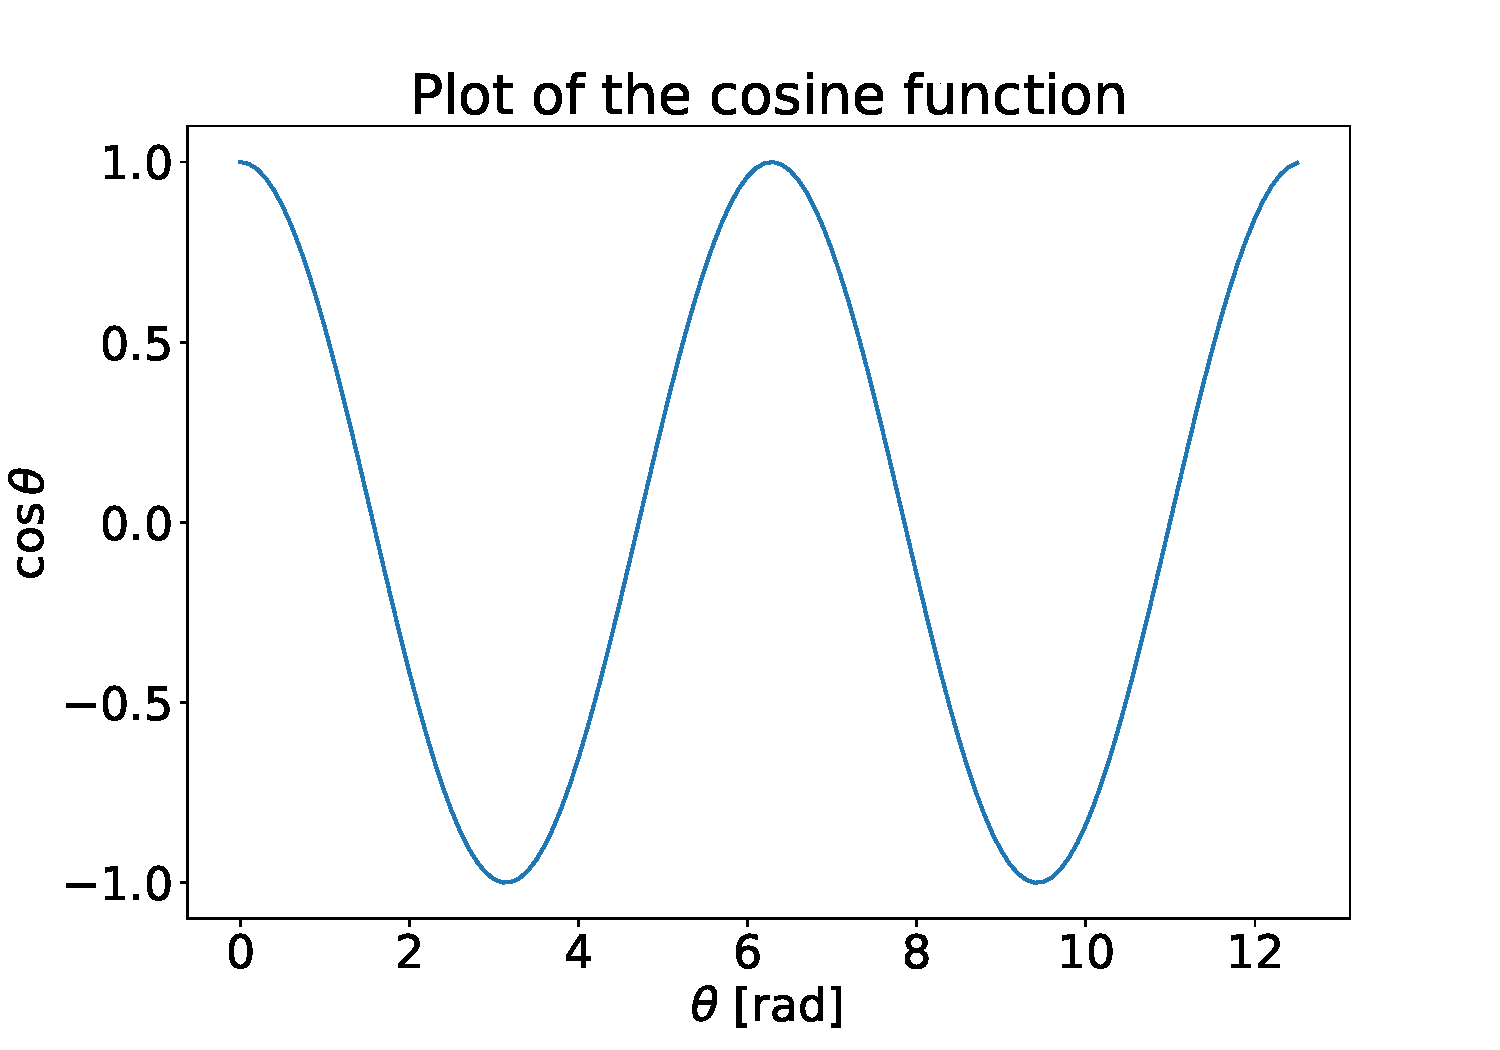
\includegraphics[width=0.5\textwidth]{figs/cos.pdf}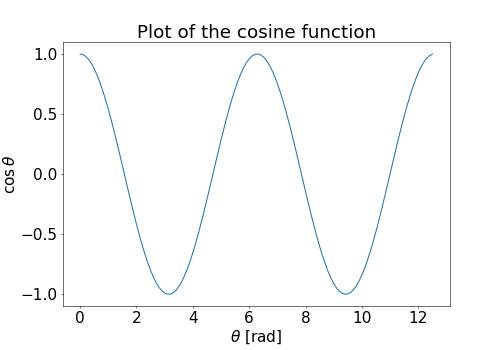
\includegraphics[width=0.5\textwidth]{figs/cos.png}
    \caption{Plot of a cosine function, included from a file in vector format (PDF, left plot) and a file in bitmap format (PNG, right plot), to illustrate the superiority in image quality of PDF over PNG}\label{fig:vectorformat}
\end{figure}


\section{Tables}\label{sec:formattables}
Tables are used to present data in an orderly manner. They can contain different kind of elements such as text, numbers and mathematical symbols and expressions. Every table must be referenced in your text, preferably before it appears. Some important aspects of a table are shown in \cref{tab:demotable} and are discussed below.

\begin{table}[htbp]\centering
  	\caption{Some important formatting aspects of a table and its caption}\label{tab:demotable}
    \begin{tikzpicture}[scale=0.8]\node at (0,0) [above right] {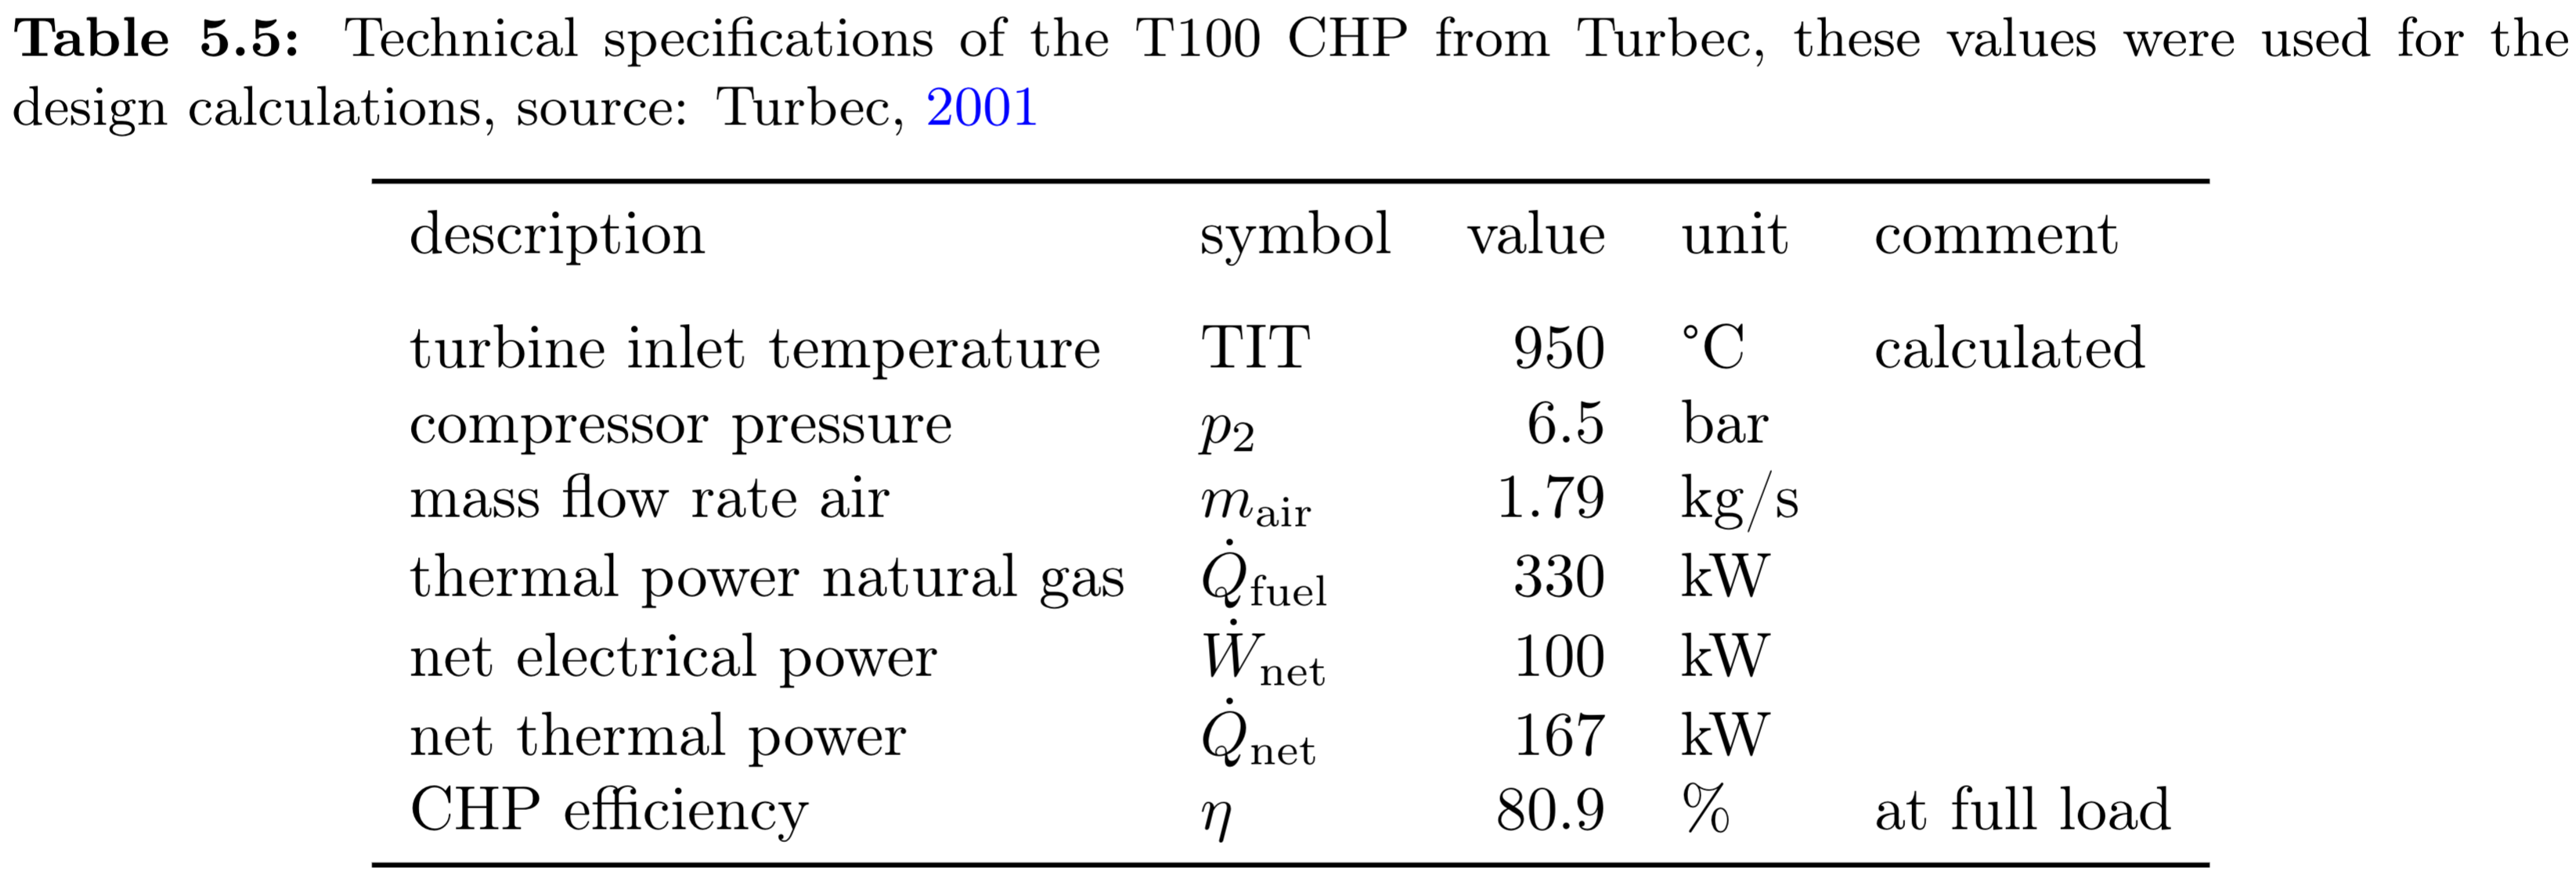
\includegraphics[width=0.9\linewidth]{figs/demotable}};
		%\draw [help lines] (0,0) grid (14,7); % uncomment to show grid
		\draw [pin] (0.4,5.8)   |- + (0.5,2)    node [right,align=left] {a numbered identifier above the table,\\referenced in the text};
		\draw [pin] (2.3,4.65)  -| + (-1,0)     node [left,align=left] {a top border};
		\draw [pin] (2.3,4.3)   -| + (-1,-0.6)  node [left,align=left] {singular column headers};
		\draw [pin] (3,3.9)   -| + (-1.2,-1.5)  node [left,align=left] {some space};
		\draw [pin] (2.3,0.3)   -| + (-1,0)     node [left,align=left] {a bottom border};
		\draw [pin] (2.3,1.5)   -| + (-0.5,0)   node [left,align=left] {a good-quality table};
	    \draw [pin] (2.4,5.8)   |- + (0.5,0.75) node [right,align=left] {a caption describing: the \textit{what}};
		\draw [pin] (11.5,5.8)  |- + (0.5,0.75) node [right,align=left] {the \textit{so-what}};
		\draw [pin] (7 ,5.1)    -| + (7.5, -2)  node [below,align=left] {the source};
		\draw [pin] ( 2.8,0.4)  -| + (0,   -1)  node [below,align=left] {text = left align};
		%\draw [pin] ( 7.8 ,0.4) -- + (0,   -1)  node [below right,align=left] {left};
		\draw [pin] (10.3 ,0.4) -- + (0,   -1)  node [below left,align=right] {number = right align};
		%\draw [pin] (10.9 ,0.4) -- + (0,   -1)  node [below right,align=left] {left};
		\draw [pin] (12.1 ,0.4) -- + (0,   -1)  node [below right,align=left] {text = left align};
	\end{tikzpicture}
\end{table}

First of all, your table must be of good quality and should provide clarity on the presented data. This means that careful consideration must be given to graphical excellence and integrity (e.g. readability, data formatting and alignment, data-ink ratio, legend,\dots).

Secondly, your table must have an unique identifier and a descriptive caption. The identifier is typically the word \texttt{Table} followed by a number. For a short report, these are typically ordinal numbers such as 1, 2, 3, etc. For a thesis or book with different chapters, the numbering of tables restarts at 1 at the beginning of each new chapter, but the chapter number is included in the table number. Table 3.2 for example refers to the second table in chapter 3. The automatic assigning of table numbers in \LaTeX\ is taken care of by the \cs{caption} command. If you want the caption to appear above the table, you must place it on the first line in the figure environment. You can inspect the source code of \cref{tab:demotable} to verify this. In Microsoft Word, captions should be added via the \texttt{insert caption} menu command.

A descriptive caption is a stand-alone text that must provide enough information to understand the data in the table, without the need to consult the text. The first word of the caption should be capitalised. The caption should contain a \textit{what} part and, if possible, a \textit{so-what} part. The \textit{what} part clearly explains what is shown in the table. Try to precise and complete, it's better to have a longer caption than a short incomplete or unclear caption. The \textit{so-what} part is a statement and explains what the reader should pay attention to and/or contains a justification for showing the table.

If you did not obtain the data in the table yourself, you must add the reference to the source of the data at the end of your caption, preceded for instance by the word \verb|source:|

If the table came from an external source but was adapted by you, you can precede the reference to the source by \verb|adapted from:|

\subsection{Header row}
A simple table will typically have a header row with a descriptor per column. Descriptors are not capitalized, unless it is required by grammar rules. Descriptors should also be written in the singular form. See for example the descriptors in \cref{tab:demo2}. You will see: parameter, value, unit, comment, and not: Parameter or Parameters or parameters,\dots

Tables can also have multiple header rows, for example a row for the descriptors and a row for the units. More complex tables can also have header columns. 

\subsection{Column alignment}
The data in the columns should be aligned. Columns that contain text should be left-aligned (column type \texttt{l}). That makes the text easier to read, because we read from left to right. See for example the improved readability of the text in the first column of \cref{tab:align1} compared to \cref{tab:align}. Columns that contain numbers should be right-aligned (column type \texttt{r}) or aligned at the decimal marker (column type \texttt{S}). This makes it easier to compare numbers in the same column as illustrated in the second column in \cref{tab:align1,tab:align}. Columns with symbols and columns with units can be centred (column type \texttt{c}), but they are easier to read when they are left-aligned.

Columns with a lot of text can become too wide, causing the table to become too wide. This can be solved by wrapping the text in the column. You can achieve this by limiting the width of a column to a specified value with the paragraph column type \texttt{p}, see example in \cref{tab:align2}.

\begin{table}\centering
    \caption{Example of a table with centered columns, which are not well suited for text and
numbers}\label{tab:align}
    \begin{tabular}{ccc}  
        \toprule
        text        &  {number}  & unit \\[1ex]
        relative humidity outside       &   62    & \% \\
        mass flow rate of fresh air     &   \num{20000}     & \unit{kg/h}\\
        total pressure at the intake of the HVAC system                        &   1   & bar\\
        \bottomrule
    \end{tabular}
\end{table}

\begin{table}\centering
    \caption{Improved table with a left-aligned text column and a right-aligned number column}\label{tab:align1}
    \begin{tabular}{lrl}  
        \toprule
        text        &  {number}  & unit \\[1ex]
        relative humidity outside       &   62    & \% \\
        mass flow rate of fresh air     &   \num{20000}     & \unit{kg/h}\\
        total pressure at the intake of the HVAC system                       &   1   & bar\\
        \bottomrule
    \end{tabular}
\end{table}

\begin{table}\centering
    \caption{A table  with wrapped text in the first column to reduce the column width}\label{tab:align2}
    \begin{tabular}{p{4.5cm}rl}  
        \toprule
        text        &  number  & unit \\[1ex]
        relative humidity outside       &   62    & \% \\
        mass flow rate of fresh air     &   \num{20000}     & \unit{kg/h}\\
        total pressure at the intake of the HVAC system                       &   1   & bar\\
        \bottomrule
    \end{tabular}
\end{table}


\subsection{Horizontal and vertical lines}
Having too many horizontal and/or vertical lines in a table is considered as visual noise and is distracting to the eye. It also lowers the data-ink ratio. Most of the time, two horizontal lines will do, one at the top of the table (\cs{toprule} command) and another at the bottom (\cs{bottomrule} command) as in \cref{tab:demotable}. These lines visually separate the data in the table from the main text. The column headers are separated from the data by some extra space. This separation can also be achieved with a horizontal line (\cs{midrule} command). Vertical lines are most of the time not required but can be added in some occasions to improve readability.

Compare for instance \cref{tab:demo1} and \cref{tab:demo2}. Both tables contain exactly the same data but \cref{tab:demo2} has the better data-ink ratio and is therefore recommended.

\begin{table}\centering
    \caption{Example of a table with unnecessary horizontal and vertical lines, giving rise to a low data-ink ratio}\label{tab:demo1}
    \begin{tabular}{|l|r|l|l|} 
        \hline
         parameter  &  value & unit         & comment\\[1.5ex]    
         \hline
         voltage    &  12   & \unit{\volt}    & given\\
         \hline
         current    &  2    & \unit{\ampere}  & given\\
         \hline
        power       &  24   & \unit{\watt}    & calculated\\
        \hline
    \end{tabular}
\end{table}

\begin{table}\centering
    \caption{Improved table with a top and a bottom line only, giving rise to an improved data-ink ratio}\label{tab:demo2}
    \begin{tabular}{lrll}  
        \toprule
         parameter  &  value & unit         & comment\\[1ex]
         voltage    &  12   & \unit{\volt}    & given\\
         current    &  2    & \unit{\ampere}  & given\\
        power       &  24   & \unit{\watt}    & calculated\\
        \bottomrule
    \end{tabular}
\end{table}

\section{Symbols}\label{sec:formatsymbols}
\subsection{Use of symbols}
Symbols are typically used to represent \emph{(physical) properties}. Physical properties play an important role in physics and engineering. Well-known physical properties are for example the mass, temperature, velocity, pressure and electric current, but there are many others.

Physical properties can be scalars (e.g. the mass $m$ and temperature $T$) but they can also be vectors (e.g. the force $\vec{F}$ and the velocity $\vec{V}$), matrices or tensors.

The value of a scalar physical properties is expressed with a number and an associated unit. One can say, for example: the ambient temperature is 298~kelvin. Note that both the name of the physical property (ambient temperature) and the name of the unit (kelvin) were written in full. That is perfectly acceptable but not so practical to use in calculations and formulas. That is why we often switch to a compact notation with \emph{symbols}.

For example, one can rewrite the statement regarding the ambient temperature as follows: the ambient temperature $ T_\up{environment}$ is 298~kelvin. Note that we used the symbol $T$ for the temperature. This is merely an agreement and  other symbols for the temperature are also possible. For example, some books use the symbol $\theta$ for the temperature. It is therefore recommended to always consult the symbol list or nomenclature of a scientific publication to find out which symbols were used. 

Useful information about the physical quantity can be mentioned in the subscript; in this example the fact that it concerns the temperature of the environment). So $_\up{environment}$ was added as a subscript to the symbol $T$.

There are also symbols for units. For example, the symbol for the kelvin is the uppercase letter K. The above statement concerning the ambient temperature can be rewritten as follows: the ambient temperature $T_\up{environment}$ = \qty{298}{\kelvin}.

\subsection{Formatting of symbols}
One-letter symbols that represent (physical) quantities -- such as for example the temperature $T$ and the voltage $U$ -- are written in italics. Everything else is written upright, as illustrated in the flowchart in \cref{fig:italics}.  Symbols that consist of more than one letter -- such as for instance the Mach number (Ma) or the Net Present Values (NPV) -- are written upright, otherwise they might be mistaken as products. That's why for instance the Reynolds number is written as Re and not as $Re$, because that could be interpreted as the product of the radius $R$ with the eccentricity $e$.

The fact that many symbols must be written upright will give you some kind of struggle, because in the math mode of \LaTeX\, letters are written in italics by default, unless you manually force them upright. The same is true for the Equation editor of Microsoft Word, there too, the standard way of writing is in italics. But no worries, how to deal with this and how to get things right is explained below.

\begin{frame}{}
    \begin{figure}\centering
        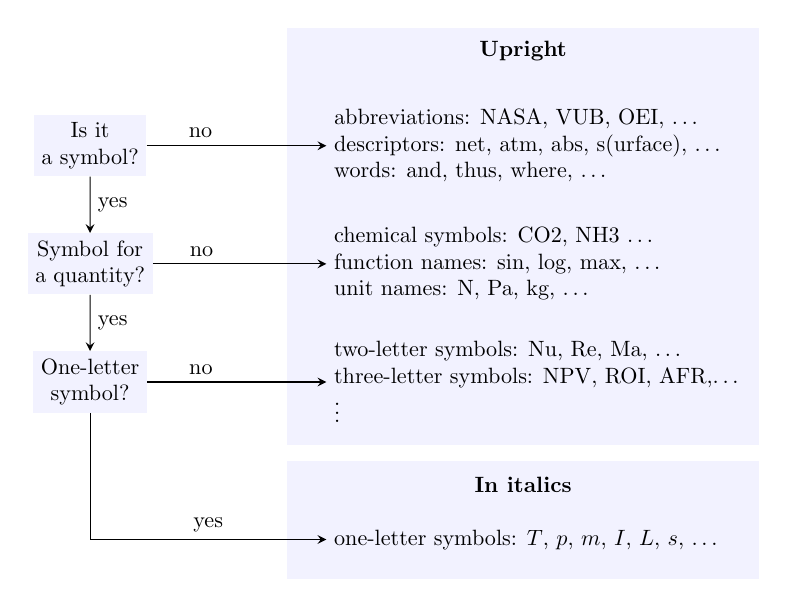
\begin{tikzpicture}[node distance=2cm,every node/.style={scale=0.8}]
            \tikzstyle{examples} = [rectangle, anchor=west,align=left]
            %\tikzstyle{decision} = [rectangle ,align=center,fill=blue!05]
            \tikzstyle{decision} = [rectangle ,align=center,fill=blue!05]
            \tikzstyle{arrow} = [thin,->,>=stealth]
            \tikzstyle{description} = [font=\bfseries]
            \tikzstyle{descriptionbox} = [fill=blue!05,align=left,right]
            %\draw [helpline] (0,0) grid (12,8);
        
            \node (symbol) [decision] at (3,5) {Is it\\ a symbol?};
            \node (quantity) [decision] at (3,3.5) {Symbol for\\ a quantity?};
            \node (oneletter) [decision] at (3,2) {One-letter\\ symbol?};
            
            \fill[descriptionbox] (5.5,1.2) rectangle (11.5,6.5);
            \fill[descriptionbox] (5.5,-0.5) rectangle (11.5,1);
            \node [description] at (8.5,6.2)  {Upright};
            \node [description] at (8.5,0.7)  {In italics};
            
            \node (nosymbol) [examples] at (6,5) {
            abbreviations: NASA, VUB, OEI, \dots\\
            descriptors: net, atm, abs, s(urface), \dots\\
            words: and, thus, where, \dots};
            
            \node (noquantity) [examples] at (6,3.5) {
            chemical symbols: \ch{CO2}, \ch{NH3} \dots\\
            function names: sin, log, max, \dots\\
            unit names: N, Pa, kg, \dots};
            
            \node (nooneletter) [examples] at (6,2) {
            two-letter symbols: Nu, Re, Ma, \dots\\
            three-letter symbols: NPV, ROI, AFR,\dots\\
            $\vdots$};
            
            \node (yesoneletter) [examples] at (6,0) {
            one-letter symbols: $T$, $p$, $m$, $I$, $L$, $s$, \dots};
            
            \draw [arrow] (symbol)   -- node[right] {yes}  (quantity);
            \draw [arrow] (quantity) -- node[right] {yes} (oneletter);
            \draw [arrow] (oneletter) |- node[above,pos=0.75] {yes} (yesoneletter);
            \draw [arrow] (symbol) -- node[above,pos=0.3] {no} (nosymbol);
            \draw [arrow] (quantity) -- node[above,pos=0.28] {no} (noquantity);
            \draw [arrow] (oneletter) -- node[above,pos=0.3] {no} (nooneletter);
        \end{tikzpicture}
        \caption{Flowchart to determine if something must be written upright or in italics: only one-letter symbols for quantities must be written in italics}\label{fig:italics}
    \end{figure}
\end{frame}

Some examples are given below and in \cref{tab:up}. So, as already mentioned, only one-letter symbols for quantities are written in italics:
\begin{align*}
    \text{correct:} \quad & T = \qty{298}{\kelvin} \\
    \text{not correct:} \quad & \up{T} = \qty{298}{\kelvin}
\end{align*}

The same goes for one-letter symbols that appear in subscripts and superscripts. The subscript $p$ for example in the specific heat capacity $c_{p}$ is written in italics because it represents a quantity:
\begin{align*}
    \text{correct:} \quad & c_{p} \quad \text{(because $p$ is a symbol for a quantity)} \\
    \text{not correct:} \quad & c_\up{p} \\
    \text{correct:} \quad & p_\up{gauge} = p_\up{abs} - p_\up{atm}\quad \text{(because the subscripts are not symbols for quantities)} \\
    \text{not correct:} \quad & p_{gauge} = p_{abs} - p_{atm}
\end{align*}

Natural constants are also quantities and their one-letter symbols are therefore also written in italics, as for example, the universal gas constant\footnote{the u in the subscript is written upright because it is not a symbol for a quantity, it's just the first letter of the word 'universal'} $R_\up{u}$ or the speed of light in vacuum $c$. 

\begin{frame}[fragile]{Some stuff is always written upright}\scriptsizebeamer
    \begin{table}\centering
    \caption{Some things are always written upright}\label{tab:up}
        \begin{tabular}{llll}
        \toprule
        type & example & \LaTeX\ example & \LaTeX\ result  \\[+1.5ex]
        %\midrule
        descriptions & abs, net, \dots & \verb|$p_\up{atm}$| & $p_\up{atm}$\\
        symbols for units & Pa, kg, \dots & \verb|\unit{\square\m}| & \unit{\square\meter}\\% see package siunitx
        math functions & log, max, \dots & \verb|$\sin\alpha$| & $\sin\alpha$\\
        chemical formulas & \ch{NH3}, \ch{CO2}, \dots & \verb|\ch{CH4}| & $\ch{CH4}$\\ % see package chemformula
        multi-letter symbols & Ma, Nu, \dots & \verb|$\up{Re}=2300$| & $\up{Re}=2300$\\
        acronyms and abbreviations & NPV, NASA, \dots & \verb|$\up{AFR}= 50$| & $\up{AFR}= 50$\\
        \bottomrule
        \end{tabular}
    \end{table}
\end{frame}

More-letter symbols for quantities are written upright:
\begin{align*}
    \text{correct:}     \quad & \up{Ma} = 0.80 \\
    \text{not correct:} \quad & Ma = 0.80 \quad \text{(undesired spacing + looks like $M$ times $a$)}\\
    \text{correct:}     \quad & \text{NPV = 3000~\euro} \\
    \text{not correct:} \quad & NPV = \text{3000~\euro} \quad \text{(undesired spacing + looks like $N$ times $P$ times $V$)}
\end{align*}

Descriptions are written upright:
\begin{align*}
    \text{correct:} \quad & T_\up{environment} = \qty{298}{\kelvin} \\
    \text{not correct:} \quad & T_{environment} = \qty{298}{\kelvin}
\end{align*}

Even if you shorten the descriptive text to make the notation more compact, you still write it upright:
\begin{align*}
    \text{correct:} \quad & T_\up{env} = \qty{298}{\kelvin} \\
    \text{not correct:} \quad & T_{env} = \qty{298}{\kelvin}
\end{align*}

Even descriptions reduced to a single letter are written upright:
\begin{align*}
    \text{correct:} \quad & T_\up{e} = \qty{298}{\kelvin}\quad \text{(because e is not a symbol for a quantity)} \\
    \text{not correct:} \quad & T_{e} = \qty{298}{\kelvin}
\end{align*}

Words are written upright, even when they appear between mathematical expressions:
\begin{align*}
    \text{correct:}     \quad &  U=I R \quad \text{with the current} \quad I=\qty{2}{\ampere}\\
    \text{not correct:} \quad &  U=I R \quad and\ the\ current \quad I=\qty{2}{\ampere}
\end{align*}

Words are written upright, even when they appear in mathematical expressions:
\begin{align*}
    \text{correct:}     \quad &   \eta=\frac{\text{work produced}}{\text{heat received}}\\
    \\
    \text{not correct:} \quad &   \eta=\frac{work\ produced}{heat\ received}
\end{align*}

Symbols for mathematical functions are written upright:
\begin{align*}
    \text{correct:}     \quad &   \sin\alpha\\
    \text{not correct:} \quad &   sin\alpha
\end{align*}

Chemical formulas are written upright:
\begin{align*}
    \text{correct:}     \quad &   \ch{CO2}\\
    \text{not correct:} \quad &       CO_2
\end{align*}

\section{Numbers}\label{sec:formatnumbers}
\subsection{Decimal marker}
We advice you to use the dot as the decimal marker for your entire document, as is common practice in English scientific literature (e.g. $\pi\approx$ 3.14).

In Belgium it is customary to use the comma as the decimal marker (e.g. $\pi\approx$ 3,14), but this will give rise to inconsistencies, as you will probably also have figures and tables from English-language literature (that contain numbers with the dot as decimal marker). Maintaining consistency in the selected decimal marker throughout your document is however essential to avoid confusing the reader. Also, the comma serves other purposes in the math mode in \LaTeX, such as for instance the separation of function arguments. For these reasons, we recommend to use the dot as the decimal marker.

\subsection{Thousands separator}
It is good practise to separate the thousands in a number with a small non-breakable space. This makes a number with many digits easier to read. The \pkg{siunitx} package can take care of this, because it provides the command \cs{num},  see \cref{sec:siunitx} for more info.

Observe for instance how the readability of the number 10 million can be improved by using the command \verb|\num{10000000}|
\begin{align*}
    \text{hard to read:}     \quad &        10000000\\
    \text{easier to read:}   \quad &   \num{10000000}
\end{align*}

Tip: do not use the comma as a thousands separator, to avoid confusion for people in Belgium who are used to the comma as a decimal marker.

\subsection{Scientific notation}
The scientific notation is used to write very large or very small numbers in a more compact form. It is also used to report numbers with the appropriate level of precision without overwhelming the reader, as illustrated in the Reynolds number example in the next subsection. Here is an example of a correctly formatted number in scientific notation: \num{6.02E23}. It consists of:
\begin{itemize}
    \item a coefficient, here: 6.02
    \item a multiplication sign, preceded and followed by a non-breaking space: $\ \times\ $
    \item a power of 10, here: \num{e23}
\end{itemize}


\subsection{Significant digits}
Calculations performed with a calculator or computer code typically produce numeric results with  many digits. But beware, it's important to understand that not all of these digits are significant. The number of significant digits depends on the uncertainty of the used input data for the calculations and on the accuracy and validity of the model(s) used in the calculations. When you include such numerical results in your report, you should only write the significant digits, being the digits that are meaningful and reliable. Writing more digits creates a false impression of precision and accuracy.

In engineering, as a rule of thumb, we typically consider 3 significant digits. But exception are of course possible. With high-precision instruments, we can perform measurements that leverage more than 3 significant digits. For instance a voltage of \qty{239.41}{\volt} with 5 significant digits. And with low-precision instruments, we get less significant digits, for instance a temperature of \qty{19}{\celsius} with only 2 significant digits. In such cases, you must of course adapt the reported number of digits accordingly.

So how to not-report the non-significant digits? Well, there are three simple methods:

\begin{enumerate}
    \item Simply not write them, but this only works for digits behind the decimal marker
    \item Switch the prefix of the unit, for instance from kWh to MWh
    \item Switch to exponential notation
\end{enumerate}

You will find an example of each method below.

Imagine that you calculated a flow velocity and obtained a value of \qty{2.385494828187}{m/s} with your calculator or computer code. Well, do not report this result will all its digits in your manuscript! Most probably, only the first 3 non-zero digits are significant. Hiding the other digits is easy, because they are located behind the decimal marker. 
\begin{align*}
    \text{not correct:} \quad & \vel = \qty{2.385494828187}{m/s} \quad \text{(too many digits, false impression of accuracy)} \\
    \text{correct:}     \quad & \vel = \qty{2.39}{m/s} \quad \text{(assuming 3 significant digits)}
\end{align*}

Imagine that you calculated the yearly heat demand of a space, based on outside temperature data (with 3 or 2 significant digits) and that your computer code produced \qty{23765.324}{kWh/year} as a result. Again, do not report this result will all its digits in your manuscript. Only the first 3 or 2 non-zero digits are significant. Hiding digits after the decimal marker is easy, but not sufficient. More digits must be hidden. We can achieve this be switching the prefix in the unit.  
\begin{align*}
    \text{not correct:} \quad & Q = \qty{23765.324}{kWh/year} \quad \text{(too many digits, false impression of accuracy)} \\
    \text{not correct:} \quad & Q = \qty{23765}{kWh/year} \quad \text{(still too many digits, false impression of accuracy)} \\
    \text{correct:}     \quad & Q = \qty{23.8}{MWh/year} \quad \text{(assuming 3 significant digits)}\\
    \text{correct:}     \quad & Q = \qty{24}{MWh/year} \quad \text{(assuming 2 significant digits)} 
\end{align*}

Imagine that you calculated the Reynolds number, based on measured flow velocity data (with 2 significant digits) and that your computer code produced $\up{Re}=\num{567214}$ as a result. You can guess, do not report this result will all its digits in your manuscript. Only the first 2 non-zero digits are significant. We can achieve this be switching to exponential notation. Switching the prefix in the unit is not an option here, because the Reynolds number has no units. 
\begin{align*}
    \text{not correct:} \quad & \up{Re} = \num{567214} \quad \text{(too many digits, false impression of accuracy)} \\
    \text{correct:}     \quad & \up{Re} = \num{5.7e5} \quad \text{(assuming 2 significant digits)} 
\end{align*}

\subsection{Uncertainty}
The uncertainty of a number can be put in parentheses behind the number \parencite[section 5.4.5]{SI}. Consider for example this length: \qty{1.236(5)}{\m}. The number in parentheses refers to the last digit of the quoted value 1.236, so in this example, the uncertainty is \qty{0.005}{\m} or \qty{5}{\mm}. An alternative notation is \qty[separate-uncertainty=true]{1.236(5)}{\m}.

\section{Units}\label{sec:formatunits}
Units must be formatted according to the International System of Units (SI) guidelines, see the rules and style conventions in section 5 of \cite{SI}. Except for dimensionless quantities, numbers without units make no sense. Units are always written upright, never in italics:
\begin{align*}
    \text{correct:} \quad & L = \qty{7}{meter} \\
    \text{not correct:} \quad & L = 7 \; meter
\end{align*}

Unit names are never capitalized unless they are at the beginning of a sentence. This is to distinguish them from the scientists they are named after. So joule is the SI unit for energy, while Joule is the name of the English physicist and mathematician James Prescott Joule. You will find examples of other unit names in Tables 2 and 4 in \cite{SI}.
\begin{align*}
    \text{correct:}     \quad & 300~\text{joule (or watt, newton, pascal, volt, bar, kelvin, \dots)} \\
    \text{not correct:} \quad & 300~\text{Joule (or Watt, Newton, Pascal, Volt, Bar, Kelvin\dots)}
\end{align*}

Special attention goes to the degree Celsius. The first word is not capitalized since the names of units are not capitalized. The second word is capitalized as it refers to the Swedish astronomer Anders Celsius. Another unit for temperature that is often used is the kelvin, written with a lowercase k, to distinguish it from the name of the British mathematician and engineer William Thomson Kelvin, also known as Lord Kelvin. It is important to note that there is no such thing as a degree Kelvin, just as there is no degree kilogram or degree meter. See the examples below.
\begin{align*}
    \text{correct:}     \quad & 0~\text{degree Celsius (small d + capital C)}\\
    \text{not correct:} \quad & 0~\text{Celsius (the word degree is missing)}\\
    \text{not correct:} \quad & 0~\text{Degree Celsius}\\
    \text{not correct:} \quad & 0~\text{degree celsius}\\
    \text{correct:}     \quad & 273~\text{kelvin}\\
    \text{not correct:}  \quad & 273~\text{Kelvin (that is the name of Lord Kelvin)}\\
    \text{not correct:} \quad & 273~\text{degree kelvin (there is no such thing as a degree kelvin)}\\
    \text{not correct:} \quad & 273~\text{degree Kelvin (there is no such thing as a degree Kelvin)}\\
\end{align*}

Symbols for units, like the letter m for meter, are always written upright:
\begin{align*}
    \text{correct:} \quad & L = \qty{7}{\meter} \\
    \text{not correct:} \quad & L = 7 \; m
\end{align*}

In this way there can be no confusion between the symbol $m$ that is used for mass and the symbol m that is used for meter. And so, for example, $A$ represents an area in \unit{\square\meter} and the A written upright represents the unit ampere for electric current.

Do not use abbreviations for units. Use the symbol or the full name:
\begin{align*}
    \text{correct:}     \quad & \text{s or second} \\
    \text{not correct:} \quad & \text{sec}\\
    \text{correct:}     \quad & \text{\unit{\m\per\s} or meter per second} \\
    \text{not correct:} \quad & \text{mps, m/sec}
\end{align*}

The symbol used for a unit is never written in the plural form:
\begin{align*}
    \text{correct:} \quad & z = \qty{120}{\centi\meter}\\
    \text{not correct:} \quad & z = 120 \; \up{cms}
\end{align*}

No full stop is put after a unit, unless that unit is at the end of a sentence:
\begin{align*}
    \text{correct:} \quad & \text{The length of the tube is 70~cm.}\\
    \text{correct:} \quad & \text{The tube is 70~cm long.} \\
    \text{not correct:} \quad & \text{The tube is 70~cm. long.}
\end{align*}

Prefixes representing a multiplication factor (\cref{t:factors}) are also written upright and written together with the symbol of the unit
\begin{align*}
    \text{correct:} \quad & \pres_\up{1} = \qty{700}{\kilo\pascal} \\
    \text{not correct:} \quad & \pres_\up{1} = 700 \, \up{k \, Pa}
\end{align*}

\begin{table}\centering
\caption{Some standard prefixes in SI units}\label{t:factors}
    \begin{tabular}{llllll}
        \toprule
        factor     & prefix & symbol     & factor     & prefix   & symbol\\[+1.5ex]
        \num{E-1}  & deci   & d          &  \num{E1}  & deca     & da \\
        \num{E-2}  & centi  & c          &  \num{E2}  & hecto    & h \\
        \num{E-3}  & milli  & m          &  \num{E3}  & kilo     & k  \\
        \num{E-6}  & micro  & \textmu    &  \num{E6}  & mega     & M\\
        \num{E-9}  & nano   & n          &  \num{E9}  & giga     & G\\
        \num{E-12} & pico   & p          &  \num{E12} & terra    & T\\
        \num{E-15} & femto  & f          &  \num{E15} & peta     & P \\
        \num{E-18} & atto   & a          &  \num{E18} & exa      & E \\
        \num{E-21} & zepto  & z          &  \num{E21} & zetta    & Z \\
        \bottomrule
    \end{tabular}
\end{table}

\subsection{Spaces}
A number must be kept together with its unit. This can be achieved by putting an unbreakable space between the number and the unit. This will 'glue' the unit to the number, so that the number doesn't end up alone at the end of a line with the unit at the start of the next line.

To achieve this in \LaTeX\ you use the tilde \verb|~| in text mode and the \verb|\;| in math mode. So for instance \verb|80~kg| will appear as 80~kg. Or even better, you can use the package \pkg{siunitx} that will take care of the proper spacing for you, amongst many other things related to numbers and units (more info in \cref{sec:siunitx}).

In Microsoft Word you must type \texttt{shift-ctrl-space} to produce an unbreakable space.

The unit can also be 'glued' to the number by suppressing the space between them, but this is considered as bad practice.
\begin{align*}
    \text{correct:} \quad & \vol =\qty{3}{\cubic\meter} \\
    \text{bad practice:} \quad & \vol = 3 \up{m ^ 3}
\end{align*}

\section{Mathematical expressions}\label{sec:formatmath}
\subsection{Equations}
It is good practice to number your equations, because it allows to cross-reference them from elsewhere in your text. Automatic numbering can be achieved by using the \texttt{equation} environment, as shown in the first law of thermodynamics for closed systems below
\begin{equation}\label{eq:1stlawclosedsystem}
    \Delta E = Q + W.
\end{equation}

To establish a cross-reference, you must first add a label to the equation environment. You can then use this label in a \cs{cref} command elsewhere. Inspect the source code of \cref{eq:1stlawclosedsystem} to see how this is done.

There are many other math-environments available in \LaTeX\ that can do more complicated things with equations such as splitting, grouping and aligning. More info is available on the Overleaf help page about \href{https://www.overleaf.com/learn/latex/Aligning_equations_with_amsmath}{aligning equations with amsmath}.

\subsection{Multiplication sign}
To write a multiplication of two variables, leave a small space between them or put a proper multiplication operator between them. In math mode in \LaTeX, use \cs{cdot} to produce the center dot $\cdot$ or use \cs{times} to produce the multiplication sign $\times$.

In Microsoft Word, you can use \cs{bullet} in the equation editor to produce the center dot $\cdot$.

Other symbols, such as the asterisk *, the letter x and the full stop, should be avoided.
\begin{frame}[fragile]{Some good and bad symbols for multiplying}
    \begin{align*}
    \text{correct:} \quad & U = I\, R \\
    \text{correct:} \quad & U = I\cdot R\\
    \text{acceptable:} \quad & U = I\times R \quad\text{might be confused with vector product}\\
    \text{bad practice:} \quad & U = I * R \\
    \text{bad practice:} \quad & U = I x R \\
    \text{bad practice:} \quad & U = I.R
    \end{align*}
\end{frame}

\subsection{Punctuation}
Equations are part of the sentence structure, which means
punctuation must be respected. See the example below.

Newton's second law is
\begin{equation}\label{eq:newton}
    \vec{F} = m \cdot \vec{a},
\end{equation}
where $\vec{F}$  is the force,  $m$ the mass and $\vec{a}$ the acceleration.

\section{Slides}\label{sec:slides}
You can also make slides with this template. To do so, select the file \texttt{mainSlides} as your main document via the Menu-button in the upper left corner in Overleaf and compile it. You will see that the first line of \texttt{mainSlides} loads the class \pkg{beamer} which is a powerful \LaTeX\ class to create presentations. More info about this class can be found on the \href{https://www.overleaf.com/learn/latex/Beamer}{Overleaf help pages on Beamer}.

In beamer, slides are called frames. When you compile \texttt{mainSlides}, \LaTeX\ will process the content that is embedded in all the frame environments and put that content on slides. Each frame environment becomes a separate slide. The syntax of a frame environment is shown in \cref{list:frame}.

% the listing below contains a \begin{frame} command. This confuses beamer. Therefor we switch to article mode first, to ignore it in the presentation modes
\mode<article>
\begin{lstlisting}[language=latexcode,style=latexstyle,label={list:frame},caption={Syntax of a frame environment}]
 \begin{frame}*\oarg{options}\marg{title of your slide}*
    %  content is provided in plain text format
 \end{frame}
\end{lstlisting}
% switch back to mode* = ignore all text outside frames in the presentation modes
\mode*


There are some things that are good to know, when making slides. They are discussed by Jean-Luc Doumont in a talk he gave at Stanford University in 2013. The video is still \href{https://youtu.be/meBXuTIPJQk?si=73K4pQiQybXcaqDS}{available on YouTube} and is worth watching. Some of his recommendations are listed below. If you inspect the source code, you will see that they are embedded in a frame environment. This means that besides being visible in this report (compiled with the class \pkg{memoir}), they will also end up on a slide (when compiled with the class \pkg{beamer}).

\begin{frame}{It is important to be aware of these guidelines when making slides}
% this slide is an example of a slide with two columns with text aligned at the top
 \begin{columns}
     \begin{column}[t]{0.4\textwidth} % resize if you wish
       A slide should:
        \begin{itemize}\setlength\itemsep{2ex} % 
            \item have a clear title
            \item have a sober background
            \item contain clear content
            \item have no unreadable text
        \end{itemize}
    \end{column}
    \begin{column}[t]{0.6\textwidth}  % resize if you wish
        A title should be:
        \begin{itemize}\setlength\itemsep{2ex} 
            \item a \textit{so-what} message, telling the reason that you are showing the slide, rather than just a \textit{what} message about the content of the slide
            \item left-aligned, because that is easier to read
            \item written as a full sentence, so with a verb, to get your message across
            \item two lines maximum, more lines will probably not be read 
        \end{itemize} 
    \end{column}
\end{columns}
\end{frame}

You can see an example in \cref{fig:demoslide}.

\begin{figure}\centering
    \begin{tikzpicture}[scale=0.8]\node at (0,0) [above right] {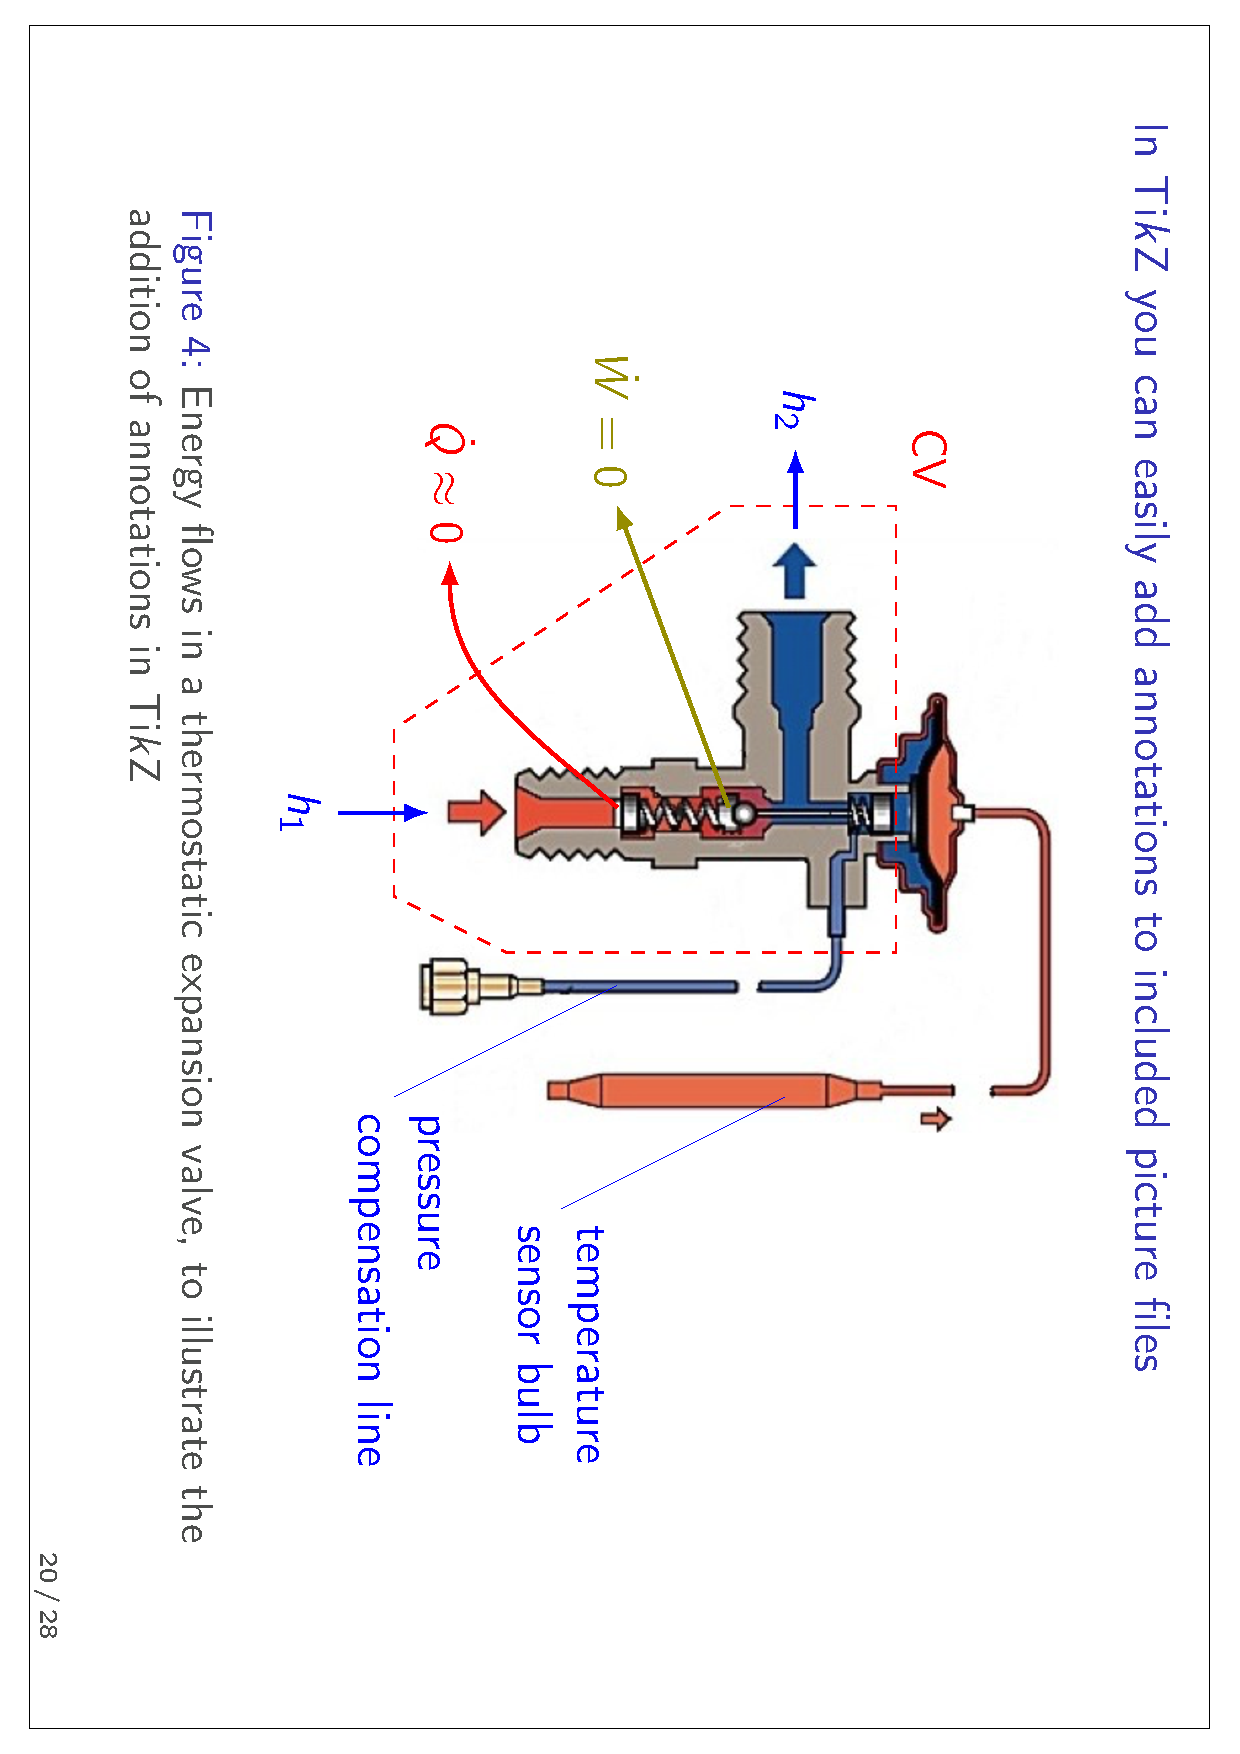
\includegraphics[angle=90,width=0.8\linewidth]{figs/demoslide}};
        %\draw [helpline] (0,0) grid (16,10); % uncomment to show grid
        \draw [pin] (1.2,10)   |- + (0.5,1) node [right,align=left] {A title with a \textit{so-what} message};
        \draw [pin] (12,7)  -- + (3,1) node [right,align=left] {sober \\background};
        \draw [pin] (12,2.5)  -- + (3,-1) node [right,align=left] {clear content,\\no unreadable text};
    \end{tikzpicture}
    \caption{An example of a slide with a \textit{so-what} message in the title, a sober background and some clear content with no unreadable text}\label{fig:demoslide}
\end{figure}

\subsection{Making content for slides only}
It is also possible to create content that will only show up on a slide, but not in your report. You can achieve this by specifying the mode \texttt{<presentation>} in the frame environment. In the source code beneath this sentence, a frame environment is specified that is invisible in this report, as you can not see :-) But it will show up on a slide, when compiled with the class \pkg{beamer}.

\begin{frame}<presentation>{It is possible to add content to a slide that is not visible in your report}
This sentence can only be seen on a slide because this frame environment has mode \texttt{<presentation>} added to its source code
\end{frame}

\subsection{Creating content in Python}
It is possible to generate content for your report and/or slides using a programming language such as Python. For instance, \cref{tab:pythontable} is entirely generated within Python with the script \texttt{scripts/capacityfactor.py} that creates the file \texttt{scripts/capacityfactor.tex}. The values presented in this table result from calculations performed in the script. By combining calculations and reporting in a single script, the need to manually input static results into your report is eliminated. The same script also generates content for a slide. Compile \texttt{mainSlides} to see this slide. Inspect the script \texttt{scripts/capacityfactor.py} and the accompanying output file \texttt{scripts/capacityfactor.tex} for more info.

FYI: with a paid Overleaf subscription you can synchronise Overleaf with Dropbox, allowing seamless two-way syncing. All your Overleaf projects will appear in your Dropbox, and vice versa. This feature allows you to semi-automate the inclusion of output generated with Python into your final PDF document, requiring only one \textbf{execute} and one \textbf{recompile}. The procedure is as follows:
\begin{enumerate}
    \item Place your Python script in the corresponding Dropbox folder of your Overleaf project, ideally in a dedicated \texttt{scripts} folder.
    \item \textbf{Execute} the Python script and save the generated tex file in the same folder as your script. The tex file will automatically sync with Overleaf within a few seconds.
    \item In Overleaf, add the following lines of code:\\
    \cs{mode<all>}\\
    \cs{input}\marg{name of generated tex file}\\
    \cs{mode*}
    \item \textbf{Recompile} your project in Overleaf to incorporate the Python-generated content into your PDF.
\end{enumerate}

\mode<all> % process all content from here on. Required, otherwise the instruction \input is not processed
% This file was created with the script capacityfactor.py
\mode* % only put content inside frame environments on slides

\begin{table}\centering
    \caption{Example of a table generated in Python}\label{tab:pythontable}
    \begin{tabular}{lrl}  
        \toprule
        parameter               &  value            & unit              \\[1ex]
        \textit{inputs:}        &                   &                   \\
        nominal power           &  \num{39}       & \unit{kW}         \\
        electricity produced    &  \num{90.4}       & \unit{MWh/year}   \\[1ex]
        \textit{calculated:}    &                   &                   \\
        capacity factor         &  \num{26.5}       & \unit{\percent}   \\
        equiv. full load hours  &  \num{2318}       & \unit{\h}         \\
        \bottomrule
    \end{tabular}
\end{table}

\begin{frame}<presentation>{Example of a slide generated in Python (with script capacityfactor.py)}
An engine with a nominal power of \qty{39}{\kW} produces \qty{90.4}{\MWh} of electricity in a year.
Calculate the capacity factor (CF) and the number of equivalent full load hours (EFLH).

\begin{align*}
    \intertext{The capacity factor}
    &\up{CF} = \frac{\qty{90}{\MWh\per\yr}}{\qty{39}{\kW}\cdot\qty{8760}{\h\per\yr}}=\qty{26.5}{\percent} 
    \intertext{Equivalent hours of full load operation}
    &\up{EFLH} = \frac{\qty{90}{\MWh\per\yr}}{\qty{39}{\kW}}=\qty{2318}{\h} 
\end{align*}
\end{frame}
 % input the file that was created with a Python script
\mode*     % process only content in frame environments from here on

\subsection{Some example slides}
Compile \texttt{mainSlides} to see examples of slide templates.

\mode<all> % consult section about \mode in usefulCommands.tex for more info
\mode*

% slide with examples of vertical text spacing
\begin{frame}<presentation>{Examples of adjusting vertical text spacing on a slides}
The quick brown fox jumps over the lazy dog. The vertical space between this and the next paragraph is set to 0.25~cm.
\vspacebeamer[0.25cm] % default is 0.5 cm vertical space

The quick brown fox jumps over the lazy dog. The vertical space between this and  the next paragraph is set to 0.5~cm.
\vspacebeamer % default is 0.5 cm vertical space

The quick brown fox jumps over the lazy dog. The vertical space between this and the next paragraph is set to 1.0~cm.
\vspacebeamer[1.0cm] % set 1.0 cm vertical space

The quick brown fox jumps over the lazy dog. The quick brown fox jumps over the lazy do. The quick brown fox jumps over the lazy dog.
\end{frame}

% slide with bullet lists
\begin{frame}<presentation>{Example of a nested bullet list with custom spacing}
\begin{itemize}\setlength\itemsep{5ex} % set spacing to 4 times height of letter x
    \item first thing to mention
    \item second thing to mention
    \item third thing to mention
    \begin{enumerate}\setlength\itemsep{1ex} % set spacing to 1 times height of letter x
        \item 
        \item 
        \item 
    \end{enumerate}
    \item last thing to mention
\end{itemize}
\end{frame}

% slide with a full-slide image
\begin{frame}<presentation>[plain]
  \begin{columns} % place figure in column to remove the left margin
    \begin{column}{\paperwidth} % column width equal to paper width
      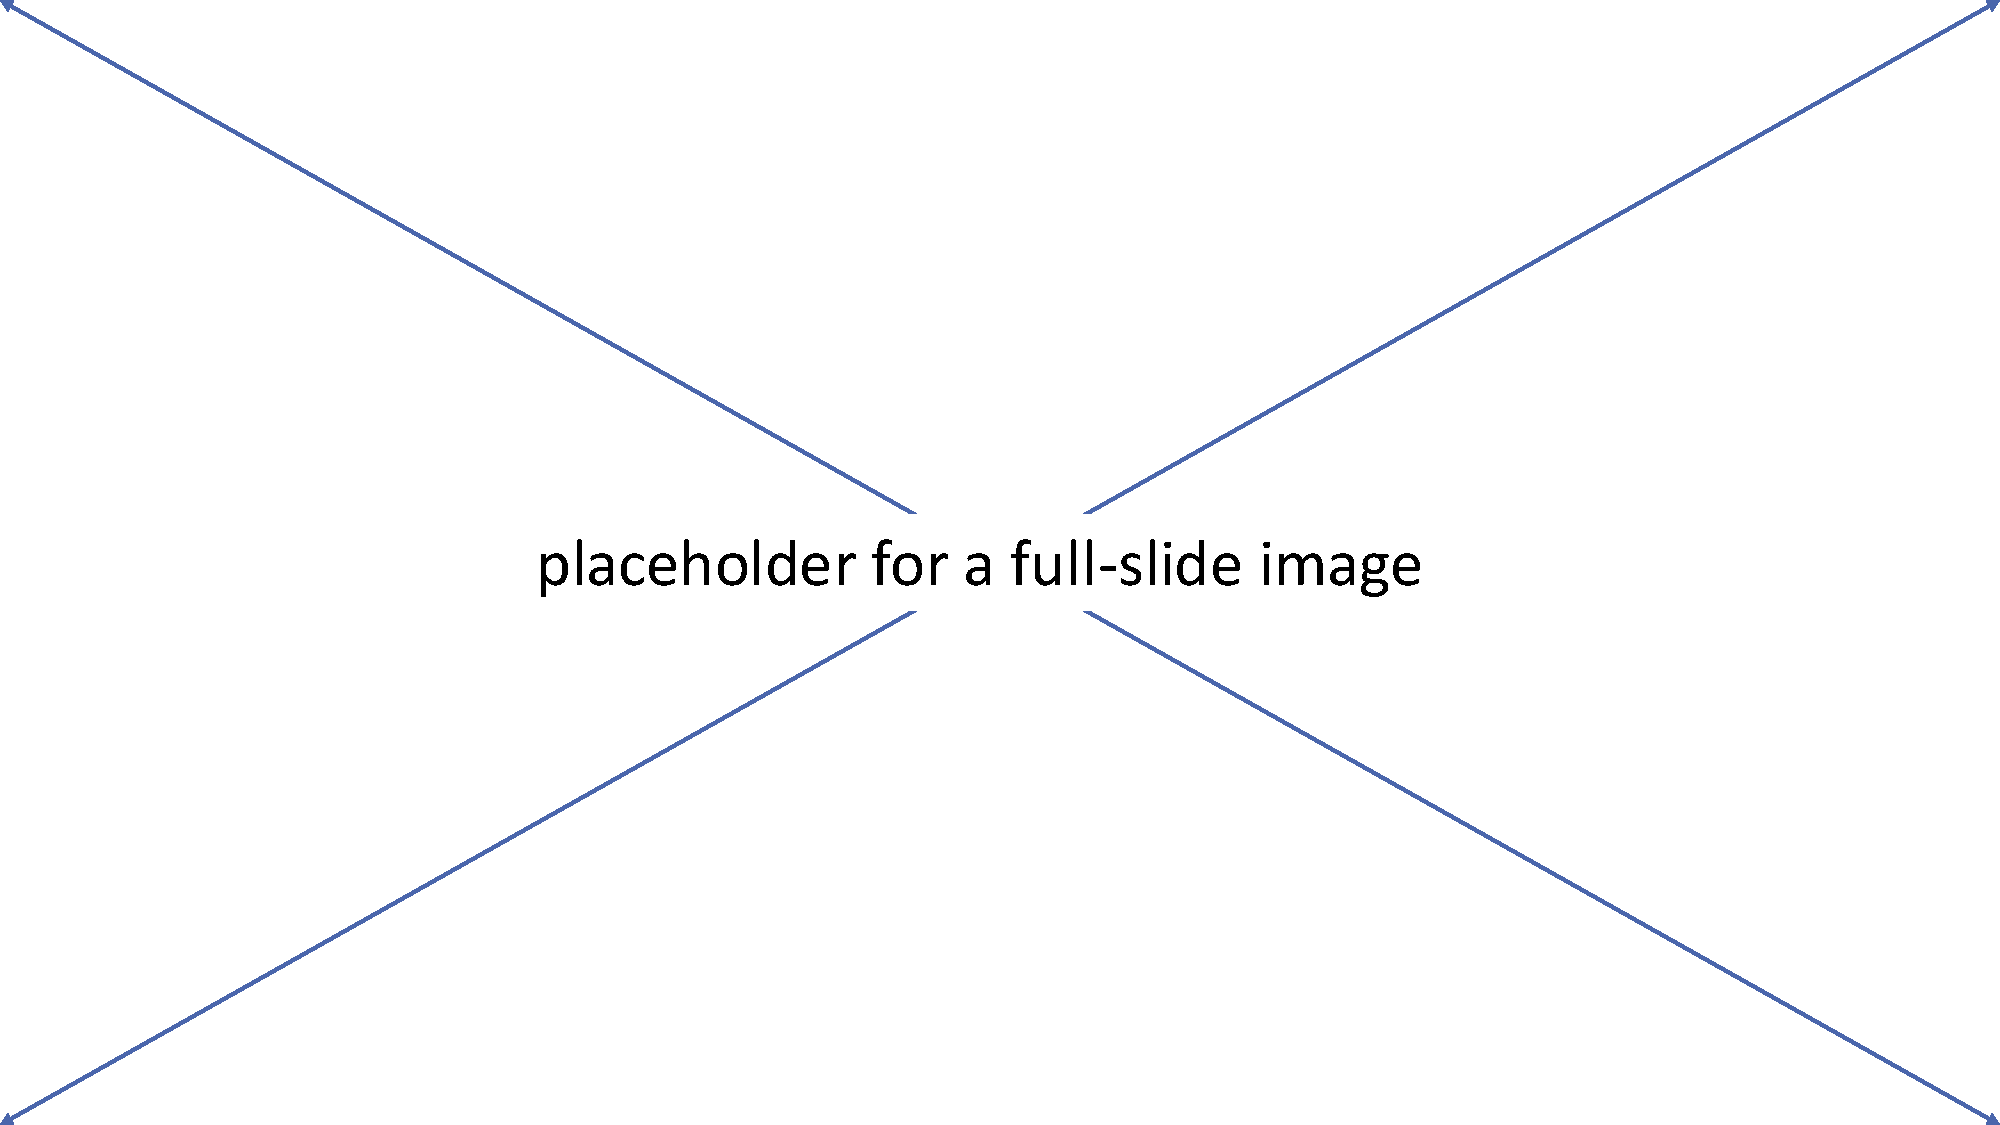
\includegraphics[height=\paperheight,width=\paperwidth]{figs/fullslideimage.pdf}
    \end{column}
  \end{columns}
\end{frame}

% slide with 2 columns
\begin{frame}<presentation>{Example of a slide with two columns}
 \begin{columns}    
    \begin{column}{0.5\textwidth} % resize if you wish
        \begin{figure}\centering
            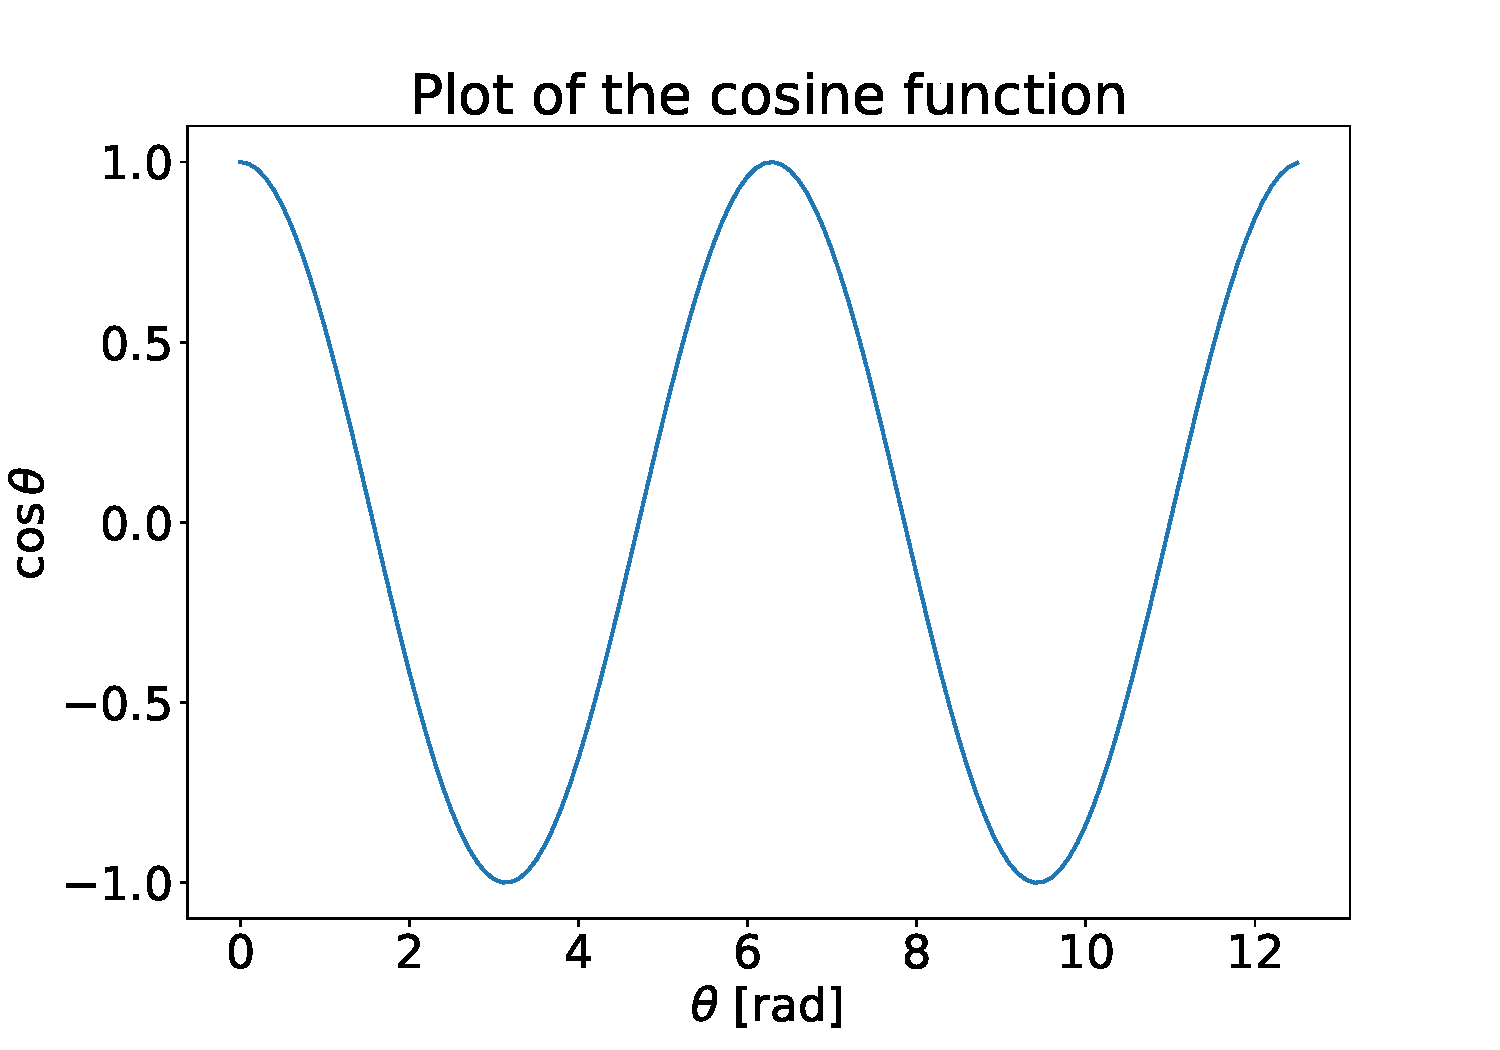
\includegraphics[width=\textwidth]{figs/cos.pdf}
            \caption{Some text}
        \end{figure}
    \end{column}
    \begin{column}{0.5\textwidth}  % resize if you wish
    \begin{align*}
        \intertext{Here you can provide extra info about the figure}
        \intertext{Equations can also easily be added}
        &\cos\theta\ \text{as function of}\ \theta
        \intertext{And some more info here}
        \intertext{And some more info here}
    \end{align*}   
    \end{column}
\end{columns}
\end{frame}

% slide with positioned blocks
% to avoid that these positioned blocks also appear in your report when compiling with memoir,
% you have to use \mode<presentation> around the frame environment
\mode<presentation>{
\begin{frame}{Example of a slide with three positioned blocks: one with a figure and two with text}
    \begin{textblock*}{7cm}(1cm,1cm)   % block width, x from left, y from top
    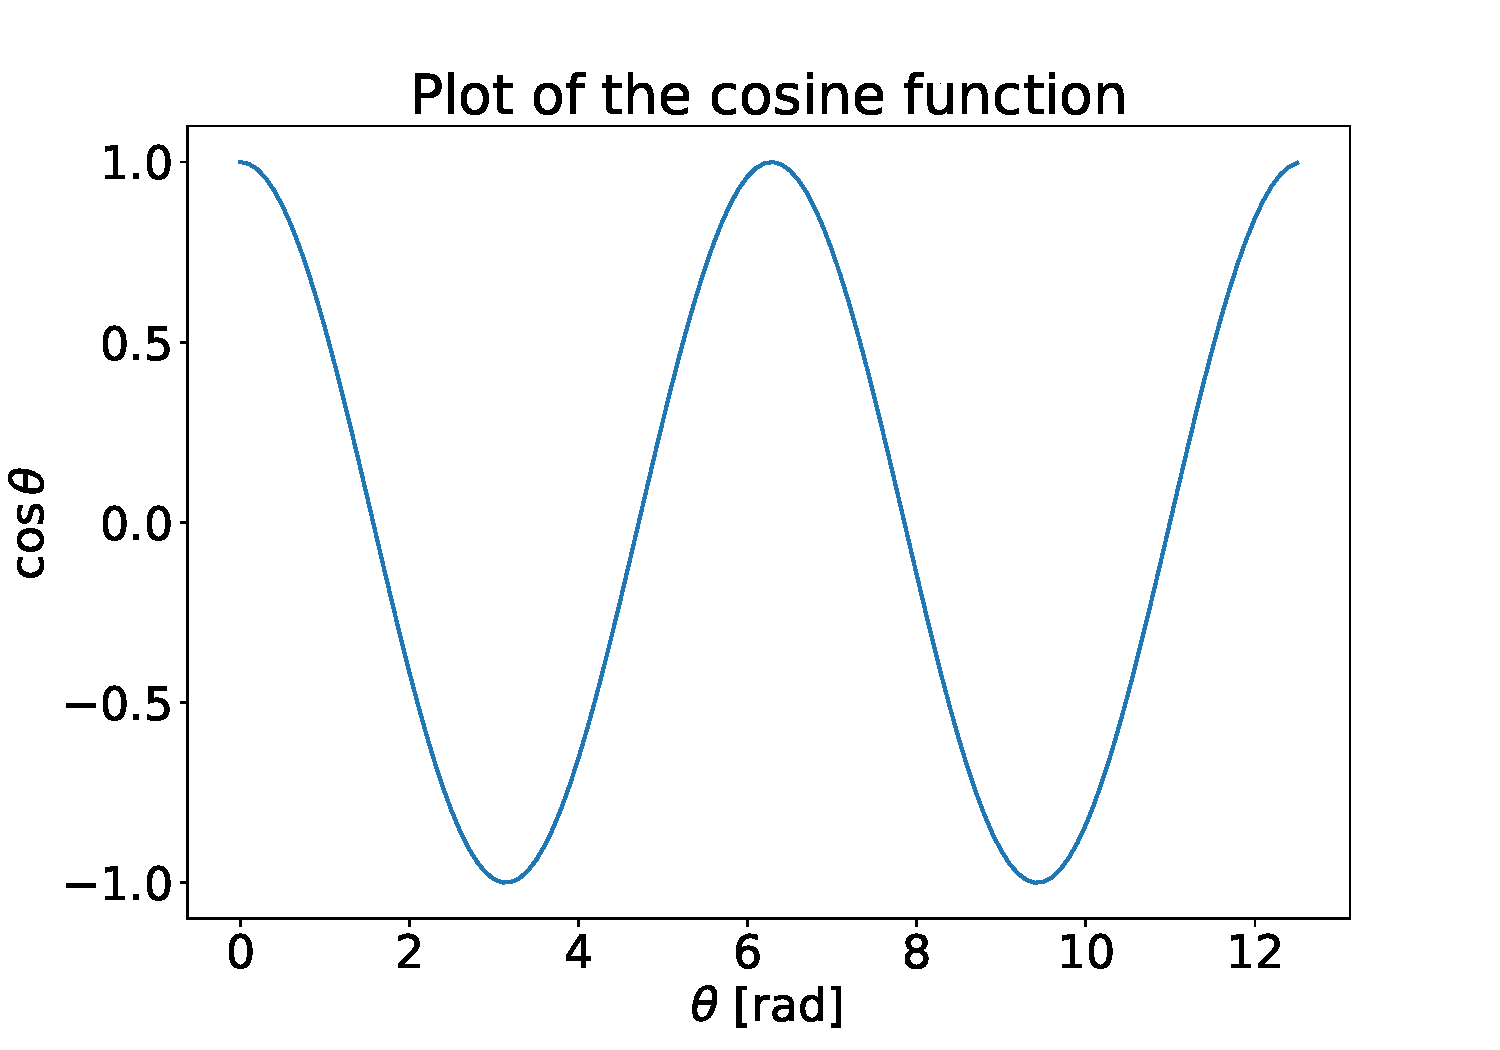
\includegraphics[width=\textwidth]{figs/cos.pdf}
    \end{textblock*}
    
    \begin{textblock*}{5cm}(8cm,2cm)   % block width, x from left, y from top
       A text block with given width positioned at location $x,y$ on the slide
    \end{textblock*}
    
    \begin{textblock*}{4cm}(3cm,6.5cm) % block width, x from left, y from top
       Another text block with given width positioned at another location $x,y$ on the slide
    \end{textblock*}
\end{frame}
}

\mode<all>


 % input the file that was created with a Python script
\mode*     % consult section about \mode in usefulCommands.tex for more info


\section{Using other people's work}\label{sec:formatcites}
In your report or thesis you will probably use information from other sources. If you do so, you have to explain to the reader where this information came from and where this information can be found. This is of great importance for the following three reasons:
\begin{enumerate}
    \item it gives proper credit to the authors or creators of your sources
    \item it allows the reader of your work to look-up and consult the source to learn more about a subject
    \item it avoids that you are being suspected of plagiarism
\end{enumerate}

\subsection{Citing}
Citing is the crediting of author(s) of a source, directly in your text. This is done by putting in-text citations in the body of your text. They are typically placed immediately after the information being cited. In \LaTeX\ we use the package \pkg{BibLaTeX} to take care of the citations, see \cref{sec:biblatex} for more info. There are three commands you should know when citing.

The \cs{cite} command is used to refer to a work itself, as part of the sentence. For example:

\begin{quotation}
The visual display of quantitative information is discussed in \cite{tufte2001}.
\end{quotation}

The \cs{textcite} command is used to refer to the author(s) of a work, as part of the sentence.
\begin{quotation}
 \textcite{tufte2001} discusses how quantitative information is visually displayed.
\end{quotation}

The \cs{parencite} command is used to cite a work when the sentence is already complete. In this case, the citation is placed in parentheses at the end of the sentence, but before the full stop. If you remove the parentheses and their content, the sentence should still make grammatical sense.
\begin{quotation}
 Quantitative information is visually displayed in different ways \parencite{tufte2001}.
\end{quotation}

A citation must always be placed inside a sentence, never behind the full stop.
\begin{align*}
    \text{correct:  }      &\text{This is a sentence [1].} \\
    \text{bad practice:  } &\text{This is a sentence. [1]}
\end{align*}



There are many different citation styles. \Cref{tab:cites} contains information on three popular citation styles (author-year, numeric and alphabetic) and shows the effect on the three cite commands that were mentioned above.

\subsection{Sources}
You should use reliable sources, such as articles from scientific journals. Wikipedia for instance, can certainly be useful as inspiration, and help you understand certain things better, but can't be regarded as primary scientific source material. It's better to consult and use the underlying sources that Wikipedia is citing. So in principle, no reference to Wikipedia should appear in your reference list. But of course exceptions are possible.

\subsection{Bibliography}
The bibliography is a list with all the cited sources in your work. It is typically placed at the very end of your document. It must contain the necessary information to find back the references. Typically: the names of the authors, the title of the work, the publication date, details of the publisher and the name of the journal.

In this template, the command \cs{printbibliography} at the end of the main file produces the bibliography. There are many different styles for a bibliography but we advise you to use one of the standard styles. As was already the case with the citations, the package \pkg{BibLaTeX} will take care of the bibliography. See \cref{sec:biblatex} for more info on this package.

\section{English}\label{sec:formatenglish}
In the European Union, British English is mostly used. American English can also be used, if there are reasons to do so. In any case, you should consistently use one type of spelling throughout your entire document, so American and British spelling cannot be mixed. Some examples of the differences between the British and American spelling are shown in \cref{tab:english}.

\begin{table}\centering
	 \caption{Some examples of words in British and American spelling; in the EU, British English is recommended}\label{tab:english}
        \begin{tabular}{ll}
            \toprule
             British        & American\\[+1.5ex]
             analyse        & analyze\\
             aerofoil       & airfoil\\
             aeroplane      & airplane\\
             aluminium      & aluminum \\
             behaviour      & behavior\\
             catalogue      & catalog \\
             centre         & center\\
             cheque         & check \\
             colour         & color\\
             defence        & defense\\
             fibre          & fiber \\
             grey           & gray \\
             initialise     & initialize\\
             labelled       & labeled\\
             licence        & license \\
             litre          & liter\\
             manoeuvre      & maneuver \\
             metre          & meter\\
             modelling      & modeling\\
             modelled       & modeled\\
             mould          & mold\\
             neighbour      & neighbor\\
             optimise       & optimize\\
             organisation   & organization \\
             parameterise   & parameterize\\
             pressurise     & pressurize\\
             programme      & program\\
             realise        & realize\\
             standardise    & standardize\\
             tonne          & ton \\
             tyre           & tire\\
             vapour         & vapor\\
             \bottomrule
        \end{tabular}
\end{table}

% more info on \mode<all> in section 21.3 of beameruserfile.pdf
\mode<all>












